\section{genericRPG.cc File Reference}
\label{genericRPG_8cc}\index{genericRPG.cc@{genericRPG.cc}}
{\tt \#include \char`\"{}genericRPG.h\char`\"{}}\par


Include dependency graph for genericRPG.cc:\nopagebreak
\begin{figure}[H]
\begin{center}
\leavevmode
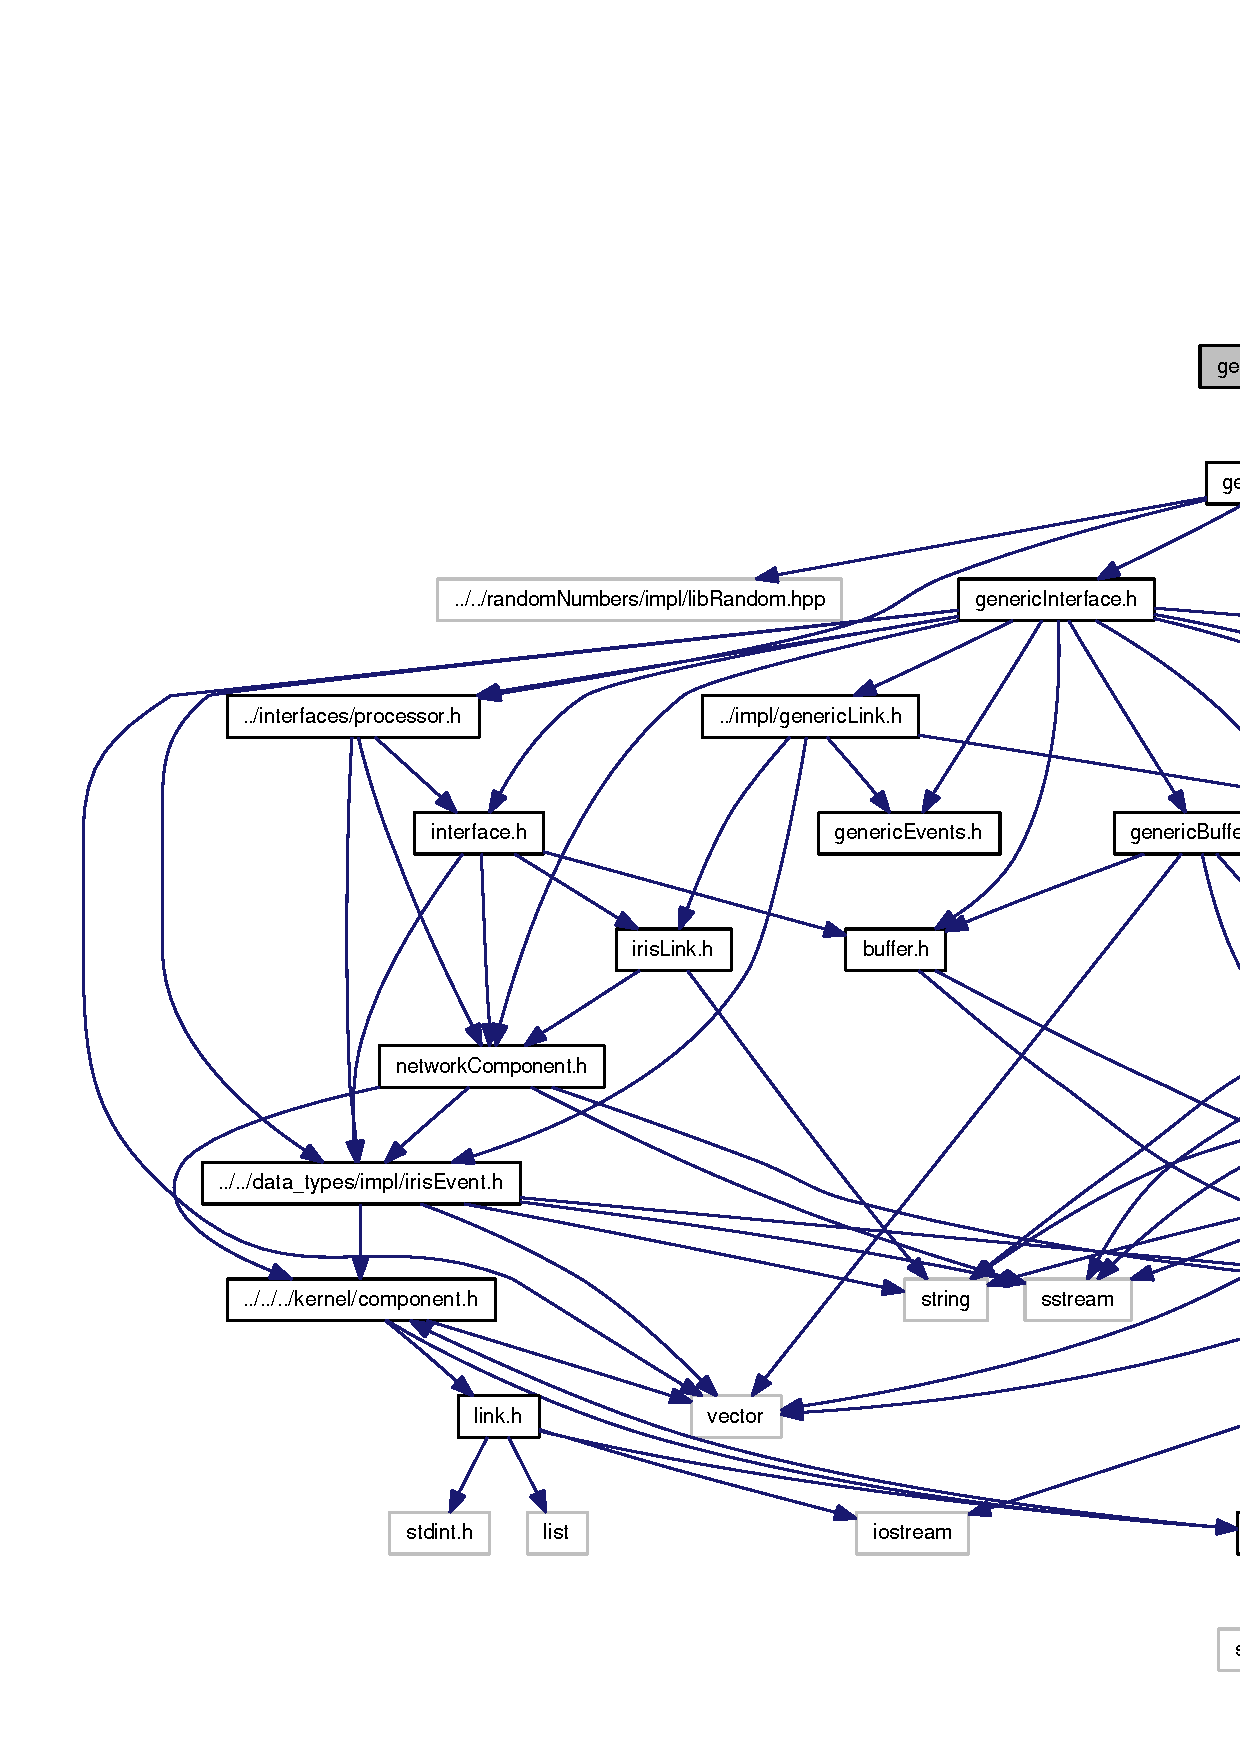
\includegraphics[width=420pt]{genericRPG_8cc__incl}
\end{center}
\end{figure}
\subsection*{Defines}
\begin{CompactItemize}
\item 
\#define {\bf MAX\_\-SIM\_\-TIME}~2000000000
\end{CompactItemize}


\subsection{Define Documentation}
\index{genericRPG.cc@{genericRPG.cc}!MAX\_\-SIM\_\-TIME@{MAX\_\-SIM\_\-TIME}}
\index{MAX\_\-SIM\_\-TIME@{MAX\_\-SIM\_\-TIME}!genericRPG.cc@{genericRPG.cc}}
\subsubsection[{MAX\_\-SIM\_\-TIME}]{\setlength{\rightskip}{0pt plus 5cm}\#define MAX\_\-SIM\_\-TIME~2000000000}\label{genericRPG_8cc_d8e040466c3a1ce9fc07153e7360ba21}




Definition at line 4 of file genericRPG.cc.

Referenced by GenericRPG::handle\_\-out\_\-pull\_\-event(), and GenericRPG::handle\_\-ready\_\-event().